\documentclass[]{article}
\usepackage{lmodern}
\usepackage{amssymb,amsmath}
\usepackage{ifxetex,ifluatex}
\usepackage{fixltx2e} % provides \textsubscript
\ifnum 0\ifxetex 1\fi\ifluatex 1\fi=0 % if pdftex
  \usepackage[T1]{fontenc}
  \usepackage[utf8]{inputenc}
\else % if luatex or xelatex
  \ifxetex
    \usepackage{mathspec}
  \else
    \usepackage{fontspec}
  \fi
  \defaultfontfeatures{Ligatures=TeX,Scale=MatchLowercase}
\fi
% use upquote if available, for straight quotes in verbatim environments
\IfFileExists{upquote.sty}{\usepackage{upquote}}{}
% use microtype if available
\IfFileExists{microtype.sty}{%
\usepackage{microtype}
\UseMicrotypeSet[protrusion]{basicmath} % disable protrusion for tt fonts
}{}
\usepackage[left=1.1in, right=1.1in, top=1.1in, bottom=1.1in]{geometry}
\usepackage{hyperref}
\hypersetup{unicode=true,
            pdftitle={Stat 435 Lecture Notes 5b},
            pdfauthor={Xiongzhi Chen; Washington State University},
            pdfborder={0 0 0},
            breaklinks=true}
\urlstyle{same}  % don't use monospace font for urls
\usepackage{color}
\usepackage{fancyvrb}
\newcommand{\VerbBar}{|}
\newcommand{\VERB}{\Verb[commandchars=\\\{\}]}
\DefineVerbatimEnvironment{Highlighting}{Verbatim}{commandchars=\\\{\}}
% Add ',fontsize=\small' for more characters per line
\usepackage{framed}
\definecolor{shadecolor}{RGB}{248,248,248}
\newenvironment{Shaded}{\begin{snugshade}}{\end{snugshade}}
\newcommand{\KeywordTok}[1]{\textcolor[rgb]{0.13,0.29,0.53}{\textbf{{#1}}}}
\newcommand{\DataTypeTok}[1]{\textcolor[rgb]{0.13,0.29,0.53}{{#1}}}
\newcommand{\DecValTok}[1]{\textcolor[rgb]{0.00,0.00,0.81}{{#1}}}
\newcommand{\BaseNTok}[1]{\textcolor[rgb]{0.00,0.00,0.81}{{#1}}}
\newcommand{\FloatTok}[1]{\textcolor[rgb]{0.00,0.00,0.81}{{#1}}}
\newcommand{\ConstantTok}[1]{\textcolor[rgb]{0.00,0.00,0.00}{{#1}}}
\newcommand{\CharTok}[1]{\textcolor[rgb]{0.31,0.60,0.02}{{#1}}}
\newcommand{\SpecialCharTok}[1]{\textcolor[rgb]{0.00,0.00,0.00}{{#1}}}
\newcommand{\StringTok}[1]{\textcolor[rgb]{0.31,0.60,0.02}{{#1}}}
\newcommand{\VerbatimStringTok}[1]{\textcolor[rgb]{0.31,0.60,0.02}{{#1}}}
\newcommand{\SpecialStringTok}[1]{\textcolor[rgb]{0.31,0.60,0.02}{{#1}}}
\newcommand{\ImportTok}[1]{{#1}}
\newcommand{\CommentTok}[1]{\textcolor[rgb]{0.56,0.35,0.01}{\textit{{#1}}}}
\newcommand{\DocumentationTok}[1]{\textcolor[rgb]{0.56,0.35,0.01}{\textbf{\textit{{#1}}}}}
\newcommand{\AnnotationTok}[1]{\textcolor[rgb]{0.56,0.35,0.01}{\textbf{\textit{{#1}}}}}
\newcommand{\CommentVarTok}[1]{\textcolor[rgb]{0.56,0.35,0.01}{\textbf{\textit{{#1}}}}}
\newcommand{\OtherTok}[1]{\textcolor[rgb]{0.56,0.35,0.01}{{#1}}}
\newcommand{\FunctionTok}[1]{\textcolor[rgb]{0.00,0.00,0.00}{{#1}}}
\newcommand{\VariableTok}[1]{\textcolor[rgb]{0.00,0.00,0.00}{{#1}}}
\newcommand{\ControlFlowTok}[1]{\textcolor[rgb]{0.13,0.29,0.53}{\textbf{{#1}}}}
\newcommand{\OperatorTok}[1]{\textcolor[rgb]{0.81,0.36,0.00}{\textbf{{#1}}}}
\newcommand{\BuiltInTok}[1]{{#1}}
\newcommand{\ExtensionTok}[1]{{#1}}
\newcommand{\PreprocessorTok}[1]{\textcolor[rgb]{0.56,0.35,0.01}{\textit{{#1}}}}
\newcommand{\AttributeTok}[1]{\textcolor[rgb]{0.77,0.63,0.00}{{#1}}}
\newcommand{\RegionMarkerTok}[1]{{#1}}
\newcommand{\InformationTok}[1]{\textcolor[rgb]{0.56,0.35,0.01}{\textbf{\textit{{#1}}}}}
\newcommand{\WarningTok}[1]{\textcolor[rgb]{0.56,0.35,0.01}{\textbf{\textit{{#1}}}}}
\newcommand{\AlertTok}[1]{\textcolor[rgb]{0.94,0.16,0.16}{{#1}}}
\newcommand{\ErrorTok}[1]{\textcolor[rgb]{0.64,0.00,0.00}{\textbf{{#1}}}}
\newcommand{\NormalTok}[1]{{#1}}
\usepackage{graphicx,grffile}
\makeatletter
\def\maxwidth{\ifdim\Gin@nat@width>\linewidth\linewidth\else\Gin@nat@width\fi}
\def\maxheight{\ifdim\Gin@nat@height>\textheight\textheight\else\Gin@nat@height\fi}
\makeatother
% Scale images if necessary, so that they will not overflow the page
% margins by default, and it is still possible to overwrite the defaults
% using explicit options in \includegraphics[width, height, ...]{}
\setkeys{Gin}{width=\maxwidth,height=\maxheight,keepaspectratio}
\IfFileExists{parskip.sty}{%
\usepackage{parskip}
}{% else
\setlength{\parindent}{0pt}
\setlength{\parskip}{6pt plus 2pt minus 1pt}
}
\setlength{\emergencystretch}{3em}  % prevent overfull lines
\providecommand{\tightlist}{%
  \setlength{\itemsep}{0pt}\setlength{\parskip}{0pt}}
\setcounter{secnumdepth}{0}
% Redefines (sub)paragraphs to behave more like sections
\ifx\paragraph\undefined\else
\let\oldparagraph\paragraph
\renewcommand{\paragraph}[1]{\oldparagraph{#1}\mbox{}}
\fi
\ifx\subparagraph\undefined\else
\let\oldsubparagraph\subparagraph
\renewcommand{\subparagraph}[1]{\oldsubparagraph{#1}\mbox{}}
\fi

%%% Use protect on footnotes to avoid problems with footnotes in titles
\let\rmarkdownfootnote\footnote%
\def\footnote{\protect\rmarkdownfootnote}

%%% Change title format to be more compact
\usepackage{titling}

% Create subtitle command for use in maketitle
\newcommand{\subtitle}[1]{
  \posttitle{
    \begin{center}\large#1\end{center}
    }
}

\setlength{\droptitle}{-2em}

  \title{Stat 435 Lecture Notes 5b}
    \pretitle{\vspace{\droptitle}\centering\huge}
  \posttitle{\par}
    \author{Xiongzhi Chen \\ Washington State University}
    \preauthor{\centering\large\emph}
  \postauthor{\par}
    \date{}
    \predate{}\postdate{}
  
\usepackage{bbm}
\usepackage{amssymb}
\usepackage{amsmath}
\usepackage{graphicx,float}

\begin{document}
\maketitle

{
\setcounter{tocdepth}{2}
\tableofcontents
}
\section{}\label{section}

\section{Different Error Measures}\label{different-error-measures}

\subsection{Hypothesis testing}\label{hypothesis-testing}

\begin{itemize}
\item
  Null hypothesis \(H_0\): natural status
\item
  Alternative hypothesis \(H_1\): status under intervention; complement
  to \(H_0\)
\item
  Test statistic \(T\), rejection region \(\mathcal{T}\) and rejection
  rule \(\mathcal{R}\): reject \(H_0\) if \(T \in \mathcal{T}\)
\item
  Type I error \(\alpha\): probability of rejecting \(H_0\) when it is
  true
\item
  Type II error \(\gamma\): probability of not rejecting \(H_0\) when
  \(H_0\) is false
\item
  Power: \(1- \gamma\)
\end{itemize}

\subsection{Example 1: One Hypothesis}\label{example-1-one-hypothesis}

\begin{itemize}
\item
  Linear model: \(E(Y) = \beta_0 + \beta_1 X\)
\item
  \(H_0: \beta_1 =0\) versus \(H_1:\beta_1 \ne 0\)
\item
  Pick type I error level \(\alpha \in (0,1)\)
\item
  Test statistic \(T\); reject \(H_0\) if \(\vert T \vert > c_{\alpha}\)
\item
  How to interpret \(\alpha\)?
\end{itemize}

\subsection{Example 2: Many Hypotheses}\label{example-2-many-hypotheses}

\begin{itemize}
\item
  Linear model:
  \(E(Y) = \beta_0 + \beta_1 X + \cdots + \beta_{m} X_{m}\)
\item
  \(H_{i0}: \beta_i =0\) versus \(H_{i1}:\beta_i \ne 0\),
  \(i=1,\ldots,m\)
\item
  Test all \(H_{i0},i=1,\ldots,m\) simultaneously
\item
  If each \(H_{i0}, i=1,\ldots,m\) is tested individually at type I
  error level \(\alpha\), what will happen to the number of rejected
  true null hypotheses?
\end{itemize}

\subsection{Family-wise error rate
(FWER)}\label{family-wise-error-rate-fwer}

\begin{itemize}
\item
  \(H_{i0}: \beta_i =0\) versus \(H_{i1}:\beta_i \ne 0\),
  \(i=1,\ldots,m\)
\item
  Rejection of a true null hypothesis is called ``false rejection''
\item
  \(V\): number of false rejections, i.e., rejected true \(H_{i0}\)'s
\item
  Family-wise error rate (FWER): \[\Pr(V \ge 1) = 1 - \Pr(V=0)\]
\item
  Control FWER: \(\Pr(V \ge 1) \le \alpha\)
\end{itemize}

\subsection{Family-wise error rate
(FWER)}\label{family-wise-error-rate-fwer-1}

\begin{itemize}
\item
  Widely used, e.g., by FDA
\item
  Good when there are only a few hypotheses to test simultaneously
\item
  Too stringent when there are many hypotheses to test simultaneously,
  and hence may suffer loss in power
\item
  What about controlling ``k-FWER'', i.e., \[\Pr(V \ge k) \le \alpha ?\]
\end{itemize}

\section{False Discovery Rate}\label{false-discovery-rate}

\subsection{False discovery rate}\label{false-discovery-rate-1}

\begin{itemize}
\item
  Allow false rejections, and hence much less stringent than FWER
\item
  Modern standard on testing many hypotheses simultaneously
\item
  Scalable to many, many hypotheses simultaneously

  \begin{itemize}
  \tightlist
  \item
    GWAS study with a few millions of hypotheses to test simultaneously
  \item
    Gene expression study with a few thousand hypotheses to test
    simultaneously
  \end{itemize}
\item
  A standard criterion in model/variable selection
\end{itemize}

\subsection{Classification table}\label{classification-table}

\begin{itemize}
\tightlist
\item
  \(H_{i0}: \beta_i =0\) versus \(H_{i1}:\beta_i \ne 0\),
  \(i=1,\ldots,m\)
\end{itemize}

\begin{center}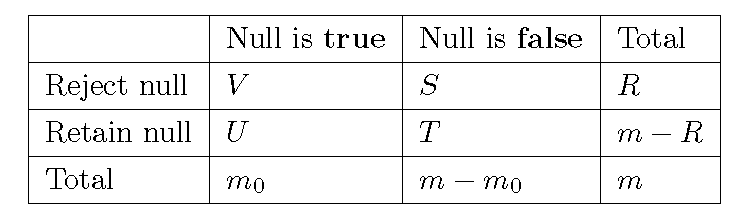
\includegraphics[width=0.85\linewidth]{classificationTable} \end{center}

\subsection{False discovery rate (FDR)}\label{false-discovery-rate-fdr}

\begin{itemize}
\item
  \(\mathcal{R}\): decision rule
\item
  \(V\): number of false rejections
\item
  \(R\): number of rejections
\item
  False discovery proportion:
  \(\mathrm{FDP}(\mathcal{R}) = V/\max\{R,1\}\)
\item
  False discovery rate:
  \[\mathrm{FDR}(\mathcal{R}) = E\left[\frac{V}{\max\{R,1\}}\right]\]
\end{itemize}

\subsection{FDR: Example}\label{fdr-example}

\begin{itemize}
\item
  \(m=5\) hypothesis \(H_{i0}: \beta_i =0, i=1,2,3,4,5\)
\item
  \(H_{i0},i=1,2,3\) are true nulls
\item
  Decision rule \(\mathcal{R}\) rejects
  \(H_{i1}, H_{i2},H_{i4}, H_{i5}\)
\item
  What is the false discovery proportion?
\end{itemize}

\subsection{Control false discovery
rate}\label{control-false-discovery-rate}

\begin{itemize}
\item
  Computing exact false discovery rate can be quite difficult
\item
  Control FDR at a nominal level:

  \begin{itemize}
  \item
    Pick a nominal level \(\alpha \in (0,1)\)
  \item
    Find a decision rule \(\mathcal{R}\), such that
    \[ \mathrm{FDR}(\mathcal{R}) \le \alpha \]
  \end{itemize}
\item
  Find such a decision rule can be hard in general
\end{itemize}

\section{Benjamini-Hochberg
procedure}\label{benjamini-hochberg-procedure}

\subsection{Benjamini-Hochberg
procedure}\label{benjamini-hochberg-procedure-1}

\begin{itemize}
\tightlist
\item
  Given: \(m\) null hypotheses \(H_{i0}\)
\item
  Given: \(m\) p-values; \(p_i\) for testing \(H_{i0}\)
\item
  Benjamini-Hochberg (BH) procedure

  \begin{itemize}
  \tightlist
  \item
    Order p-values into \(p_{(1)} \le p_{(2)} \le \cdots \le p_{(m)}\)
  \item
    Set
    \(r = \max \left\{ k \in \{1,\ldots,m \}: p_{(i)} \le i \alpha m^{-1} \right\}\)
  \item
    Rejection rule:

    \begin{itemize}
    \tightlist
    \item
      If \(r\) is defined, reject the \(r\) \(H_{i0}\)'s corresponding
      to \(p_{(1)},\ldots,p_{(r)}\)
    \item
      If \(r\) is not defined, do not reject any \(H_{i0}\)
    \end{itemize}
  \end{itemize}
\item
  Under some conditions, FDR of BH procedure is upper bounded by
  \(\alpha\)
\end{itemize}

\subsection{BH procedure: example}\label{bh-procedure-example}

\begin{itemize}
\item
  \(5\) hypotheses \(H_{10}, H_{20},H_{30},H_{40},H_{50}\)
\item
  \(p_1 = 0.03\), \(p_2 = 0.1\), \(p_3 = 0.02\), \(p_4 = 0.05\),
  \(p_5 = 0.02\)
\item
  Implement BH procedure at nominal FDR level \(\alpha =0.05\)
\end{itemize}

\section{Post-selection inference}\label{post-selection-inference}

\subsection{Linear model and LASSO}\label{linear-model-and-lasso}

\begin{itemize}
\item
  Model:
  \[Y=\beta_0+\beta_1 X_1 + \beta_2 X_2 + \ldots + \beta_p X_p + \varepsilon\]
\item
  The LASSO estimate
  \(\hat{\boldsymbol{\beta}}^L_{\lambda}=(\hat{\beta}_1,\ldots,\hat{\beta}_p)\)
  is the \({\boldsymbol{\beta}}=({\beta}_1,\ldots,{\beta}_p)\) that
  minimizes \[
  L_1(\beta_0,\boldsymbol{\beta},\lambda)= \frac{1}{2}\sum_{i=1}^n (y_i - \hat{y}_i)^2 + \lambda \sum_{i=1}^p\vert \beta_i \vert
  \]
\item
  The optimal value \(\lambda^{\ast}\) of the tuning parameter
  \(\lambda\) is often determined by \(k\)-fold cross-validation
\end{itemize}

\subsection{Linear Ridge regression}\label{linear-ridge-regression}

\begin{itemize}
\item
  Model:
  \[Y=\beta_0+\beta_1 X_1 + \beta_2 X_2 + \ldots + \beta_p X_p + \varepsilon\]
\item
  The LASSO estimate
  \(\hat{\boldsymbol{\beta}}^R_{\lambda}=(\hat{\beta}_1,\ldots,\hat{\beta}_p)\)
  is the \({\boldsymbol{\beta}}=({\beta}_1,\ldots,{\beta}_p)\) that
  minimizes \[
  L_1(\beta_0,\boldsymbol{\beta},\lambda)= \frac{1}{2}\sum_{i=1}^n (y_i - \hat{y}_i)^2 + \lambda \sum_{i=1}^p  \beta_i^2
  \]
\item
  The optimal value \(\lambda^{\ast}\) of the tuning parameter
  \(\lambda\) is often determined by \(k\)-fold cross-validation
\end{itemize}

\subsection{Penalized logistic
regression}\label{penalized-logistic-regression}

\begin{itemize}
\tightlist
\item
  LASSO logistic regression when some \(\beta_{i}\)'s are zero: \[
  \hat{\beta}=\left(  \hat{\beta}_{0},\hat{\beta}_{1},\ldots,\hat{\beta}
  _{m}\right)  \in\operatorname*{argmin}_{\beta}\left[ -\log L\left(  \beta\right)
  +\lambda\sum_{j=1}^{m}\left\vert \beta_{j}\right\vert \right]
  \]
\item
  Ridge logistic regression: \[
  \hat{\beta}=\left(  \hat{\beta}_{0},\hat{\beta}_{1},\ldots,\hat{\beta}
  _{m}\right)  \in\operatorname*{argmin}_{\beta}\left[ - \log L\left(  \beta\right)
  +\lambda\sum_{j=1}^{m}\left\vert \beta_{j}\right\vert ^{2}\right]
  \]
\item
  The optimal value \(\lambda^{\ast}\) of the tuning parameter
  \(\lambda\) is often determined by \(k\)-fold cross-validation
\end{itemize}

\textbf{Note:} \(\operatorname*{argmin}_{\beta}\) refers to optimal
\(\beta^{\ast}\) which minimizes the corresponding objective function

\subsection{Post-selection inference}\label{post-selection-inference-1}

\begin{itemize}
\item
  Post-selection inference often aims at controlling false discovery
  rate (FDR)
\item
  Benjamini-Hochberg procedure is used to control FDR
\item
  Bias correction method or knock-off method can be used
\end{itemize}

\textbf{Note:} Please see practice files

\subsection{License and session
Information}\label{license-and-session-information}

\href{http://math.wsu.edu/faculty/xchen/stat412/LICENSE.html}{License}

\begin{Shaded}
\begin{Highlighting}[]
\NormalTok{>}\StringTok{ }\KeywordTok{sessionInfo}\NormalTok{()}
\NormalTok{R version }\FloatTok{3.5.0} \NormalTok{(}\DecValTok{2018-04-23}\NormalTok{)}
\NormalTok{Platform:}\StringTok{ }\NormalTok{x86_64-w64-mingw32/}\KeywordTok{x64} \NormalTok{(}\DecValTok{64}\NormalTok{-bit)}
\NormalTok{Running under:}\StringTok{ }\NormalTok{Windows }\DecValTok{10} \KeywordTok{x64} \NormalTok{(build }\DecValTok{19045}\NormalTok{)}

\NormalTok{Matrix products:}\StringTok{ }\NormalTok{default}

\NormalTok{locale:}
\NormalTok{[}\DecValTok{1}\NormalTok{] LC_COLLATE=English_United States}\FloatTok{.1252} 
\NormalTok{[}\DecValTok{2}\NormalTok{] LC_CTYPE=English_United States}\FloatTok{.1252}   
\NormalTok{[}\DecValTok{3}\NormalTok{] LC_MONETARY=English_United States}\FloatTok{.1252}
\NormalTok{[}\DecValTok{4}\NormalTok{] LC_NUMERIC=C                          }
\NormalTok{[}\DecValTok{5}\NormalTok{] LC_TIME=English_United States}\FloatTok{.1252}    

\NormalTok{attached base packages:}
\NormalTok{[}\DecValTok{1}\NormalTok{] stats     graphics  grDevices utils     datasets  methods  }
\NormalTok{[}\DecValTok{7}\NormalTok{] base     }

\NormalTok{other attached packages:}
\NormalTok{[}\DecValTok{1}\NormalTok{] knitr_1}\FloatTok{.21}

\NormalTok{loaded via a }\KeywordTok{namespace} \NormalTok{(and not attached):}
\StringTok{ }\NormalTok{[}\DecValTok{1}\NormalTok{] compiler_3}\FloatTok{.5.0}  \NormalTok{magrittr_1}\FloatTok{.5}    \NormalTok{tools_3}\FloatTok{.5.0}    
 \NormalTok{[}\DecValTok{4}\NormalTok{] htmltools_0}\FloatTok{.3.6} \NormalTok{yaml_2}\FloatTok{.2.0}      \NormalTok{Rcpp_1}\FloatTok{.0.12}    
 \NormalTok{[}\DecValTok{7}\NormalTok{] stringi_1}\FloatTok{.2.4}   \NormalTok{rmarkdown_1}\FloatTok{.11}  \NormalTok{stringr_1}\FloatTok{.3.1}  
\NormalTok{[}\DecValTok{10}\NormalTok{] xfun_0}\FloatTok{.4}        \NormalTok{digest_0}\FloatTok{.6.18}   \NormalTok{evaluate_0}\FloatTok{.13}  
\end{Highlighting}
\end{Shaded}


\end{document}
